\documentclass{article}

\usepackage[colorlinks, urlcolor=blue, linkcolor=red, citecolor=green]{hyperref}
\usepackage{fancyhdr} %设置页眉和页脚的
\usepackage{extramarks} %设置continue那玩意的
\usepackage{amsmath}
\usepackage{amsthm}
\usepackage{amsfonts}
\usepackage{tikz} %画线的
\usepackage[plain]{algorithm}
\usepackage{algpseudocode}
\usepackage{enumerate}

\usetikzlibrary{automata,positioning}

%表
\usepackage{booktabs}
\usepackage{multirow}
\usepackage{array}
\usepackage{caption}
\DeclareCaptionFont{heiti}{\heiti} %还可以定义其他的
\captionsetup{labelsep=space, font={small, bf}, skip=2pt} %space可以改成quad

%图
%*****************图片及其相关设置***************************
\usepackage{graphicx}
\graphicspath{{tupian/}}
\usepackage{subfigure}
% 导入tikz包
\usepackage{tikz}
\usetikzlibrary{math}

%*****************代码相关设置***************************
\usepackage{pythonhighlight}
%
% Basic Document Settings
%

\topmargin=-0.45in
\evensidemargin=0in
\oddsidemargin=0in
\textwidth=6.5in
\textheight=9.0in
\headsep=0.25in

\linespread{1.1}

\pagestyle{fancy}
\lhead{\hmwkAuthorName}
\chead{\hmwkClass: \hmwkTitle}
\rhead{\firstxmark}
\lfoot{\lastxmark}
\cfoot{\thepage}

\renewcommand\headrulewidth{0.4pt}
\renewcommand\footrulewidth{0.4pt}

\setlength\parindent{0pt}

%
% Create Problem Sections
%

\newcommand{\enterProblemHeader}[1]{
    \nobreak\extramarks{}{Problem \arabic{#1} continued on next page\ldots}\nobreak{}
    \nobreak\extramarks{Problem \arabic{#1} (continued)}{Problem \arabic{#1} continued on next page\ldots}\nobreak{}
}

\newcommand{\exitProblemHeader}[1]{
    \nobreak\extramarks{Problem \arabic{#1} (continued)}{Problem \arabic{#1} continued on next page\ldots}\nobreak{}
    \stepcounter{#1}
    \nobreak\extramarks{Problem \arabic{#1}}{}\nobreak{}
}

\setcounter{secnumdepth}{0}
\newcounter{partCounter}
\newcounter{homeworkProblemCounter}
\setcounter{homeworkProblemCounter}{1}
\nobreak\extramarks{Problem \arabic{homeworkProblemCounter}}{}\nobreak{}

\newenvironment{homeworkProblem}{
    \section{Problem \arabic{homeworkProblemCounter}}
    \setcounter{partCounter}{1}
    \enterProblemHeader{homeworkProblemCounter}
}{
    \exitProblemHeader{homeworkProblemCounter}
}

%
% Homework Details
%   - Title
%   - Due date
%   - Class
%   - Section/Time
%   - Instructor
%   - Author
%

\newcommand{\hmwkTitle}{Homework\ \#1}
\newcommand{\hmwkDueDate}{March 7, 2021}
\newcommand{\hmwkClass}{Deep Learning}
\newcommand{\hmwkClassTime}{}
\newcommand{\hmwkClassInstructor}{Professor Zhen Li}
\newcommand{\hmwkAuthorName}{Peng Deng}
\newcommand{\hmwkAuthorSchool}{School of Data Science}
\newcommand{\hmwkAuthorNumber}{Sno.220041042}
%
% Title Page
%

\title{
    \vspace{2in}
    \textmd{\textbf{\hmwkClass:\ \hmwkTitle}}\\
    \normalsize\vspace{0.1in}\small{Due\ on\ \hmwkDueDate}\\
    \vspace{0.1in}\large{\textit{\hmwkClassInstructor\ \hmwkClassTime}}
    \vspace{3in}
}

\author{\textbf{\hmwkAuthorName}}


\date{}

\renewcommand{\part}[1]{\textbf{\large Part \Alph{partCounter}}\stepcounter{partCounter}\\}

%
% Various Helper Commands
%

% Useful for algorithms
\newcommand{\alg}[1]{\textsc{\bfseries \footnotesize #1}}
\usepackage[algo2e,vlined,ruled]{algorithm2e}

% For derivatives
\newcommand{\deriv}[1]{\frac{\mathrm{d}}{\mathrm{d}x} (#1)}

% For partial derivatives
\newcommand{\pderiv}[2]{\frac{\partial}{\partial #1} (#2)}

% Integral dx
\newcommand{\dx}{\mathrm{d}x}

% Alias for the Solution section header
\newcommand{\solution}{\textbf{\large Solution}}

% Probability commands: Expectation, Variance, Covariance, Bias
\newcommand{\E}{\mathrm{E}}
\newcommand{\Var}{\mathrm{Var}}
\newcommand{\Cov}{\mathrm{Cov}}
\newcommand{\Bias}{\mathrm{Bias}}
\begin{document}

\maketitle
\thispagestyle{empty}

\newpage
\setcounter{page}{1}

\begin{homeworkProblem}
Cross entropy is often used as the objective function when training neural networks in 
classification problems. Suppose the training set includes $N$ training pairs 
$D=\left\{\left(\boldsymbol{x}_{i}^{(\text {train})}, y_{i}^{(\text {train})}\right)\right\}_{i=1}^{N},$ 
where $\boldsymbol{x}_{i}^{(\text {train})}$ is a training sample and $y_{i}^{(\text {train})} \in\{1, \ldots, c\}$ 
is its corresponding class label. $\boldsymbol{z}_{i}$ is the output of the network given input $\boldsymbol{x}_{i}^{(\text {train})}$ and
the nonlinearity of the output layer is softmax. $\boldsymbol{z}_{i}$ is a $c$ dimensional vector, 
$z_{i, k} \in[0,1]$ and $\sum_{k=1}^{c} z_{i, k}=1 .$ The questions are as follows.
\begin{enumerate}[\quad(1)]
    \item Write the objective function of cross-entropy with softmax activation function, and calculate 
    the gradient of hidden-to-output and input-to-hidden weights as we introduced in class.

    \item Verify it is equivalent to the negative log-likelihood on the training set, assuming the training samples are independent.
\end{enumerate}
	
\vspace{4pt}
\textbf{\large{Solution}}

\vspace{4pt}
\textbf{Subproblem (1)}

We use one-hot encoding to encode the target value for the training sample $\boldsymbol{x}_i^{(\text {train})}$ as $\boldsymbol{t}_i (i=1,2,\dots N)$, which is 
a $c$ dimensional vector. Besides, it is defined as follows
\begin{equation}
    t_{i,k}=
    \begin{cases}
        1 & (k = y_i^{(\text {train})})\\
        0 & (k \neq y_i^{(\text {train})})
    \end{cases}
\end{equation}

\begin{enumerate}[$\circ$]
    \item The objective function can be written as follow. We use $\boldsymbol{W}$ to denote all the weights in the network.
    \begin{equation}
        \label{eq1}
        J\left(\boldsymbol{W}\right) = -\frac{1}{N}\sum_{i=1}^{N}\sum_{k=1}^{c}t_{i,k}\operatorname{log}\left(z_{i,k}\right)
    \end{equation}

    \item The gradient of hidden-to-output weights is calculated as follow. We use $net$ to denote the net value in the output layer. We set $\delta$ to denote the sensitivity in the output layer. We use $w$ to denote the weights of hidden-to-output.
    \begin{equation}
        \label{eq3}
        \begin{split}
            \frac{\partial J}{\partial w_{kj}} &= \sum_{i=1}^{N}\frac{\partial J}{\partial net_{i,k}} \frac{\partial net_{i,k}}{\partial w_{kj}}\\
            &=\sum_{i=1}^{N}-\delta_{i,k} \frac{\partial net_{i,k}}{\partial w_{kj}}\\
        \end{split}
    \end{equation}
    Then, we can calculate $\delta_{i,k}$ ans $\boldsymbol{\delta}_{i}$  as follow
    \begin{equation}
        \begin{split}
            \delta_{i,k}&=-\frac{\partial J}{\partial net_{i,k}} =-\frac{\partial J}{\partial z_{i,k}}\frac{\partial z_{i,k}}{\partial net_{i,k}}\\
            \boldsymbol{\delta}_i &=-\frac{\partial J}{\partial \boldsymbol{net}_{i}} =-\frac{\partial J}{\partial \boldsymbol{z}_{i}}\frac{\partial \boldsymbol{z}_{i}}{\partial \boldsymbol{net}_{i}}\\
        \end{split}
    \end{equation}
    Set $m = y_i^{(\text {train})}$, then we have $t_{i,m}=1$, and $\boldsymbol{t}_i = \left(0,\cdots, 1, \cdots, 0\right)$. Then we can get $\frac{\partial J}{\partial \boldsymbol{z}_{i}} $ as follow
    \begin{equation}
        \label{eq5}
        \begin{split}
            \frac{\partial J}{\partial \boldsymbol{z}_{i}} &= 
            \begin{pmatrix}
                \frac{\partial J}{\partial z_{i,1}} & \frac{\partial J}{\partial z_{i,2}} &\cdots &\frac{\partial J}{\partial z_{i,c}}
            \end{pmatrix}\\
            &=
            \begin{pmatrix}
                0&0&\cdots &-\frac{1}{N}\frac{1}{z_{i,m}}&\cdots&0
            \end{pmatrix}
        \end{split}
    \end{equation}
    Then we can calculate $\frac{\partial \boldsymbol{z}_{i}}{\boldsymbol{net}_{i}}$ as follow
    \begingroup
        \renewcommand*{\arraystretch}{1.5} 
        \begin{equation}
            \label{eq6}
            \begin{split}
                \frac{\partial \boldsymbol{z}_{i}}{\boldsymbol{net}_{i}} &= 
                \begin{pmatrix}
                    \frac{\partial z_{i,1}}{\partial net_{i,1}} & \frac{\partial z_{i,1}}{\partial net_{i,2}} & \cdots & \frac{\partial z_{i,1}}{\partial net_{i,m}}&\cdots& \frac{\partial z_{i,1}}{\partial net_{i,c}}\\
                    \vdots & \vdots & \ddots & \vdots &\ddots&\vdots\\
                    \frac{\partial z_{i,m}}{\partial net_{i,1}} & \frac{\partial z_{i,m}}{\partial net_{i,2}} & \cdots & \frac{\partial z_{i,m}}{\partial net_{i,m}}&\cdots& \frac{\partial z_{i,m}}{\partial net_{i,c}}\\
                    \vdots & \vdots & \ddots & \vdots &\ddots&\vdots\\
                    \frac{\partial z_{i,c}}{\partial net_{i,1}} & \frac{\partial z_{i,c}}{\partial net_{i,2}} & \cdots & \frac{\partial z_{i,c}}{\partial net_{i,m}}&\cdots& \frac{\partial z_{i,c}}{\partial net_{i,c}}\\
                \end{pmatrix}\\
                &=
                \begin{pmatrix}
                    \frac{\partial z_{i,1}}{\partial net_{i,1}} & \frac{\partial z_{i,1}}{\partial net_{i,2}} & \cdots & \frac{\partial z_{i,1}}{\partial net_{i,m}}&\cdots& \frac{\partial z_{i,1}}{\partial net_{i,c}}\\
                    \vdots & \vdots & \ddots & \vdots &\ddots&\vdots\\
                    -z_{i,m}\cdot z_{i,1} & -z_{i,m}\cdot z_{i,2} & \cdots &z_{i,m}-z_{i,m}^2&\cdots& -z_{i,m}\cdot z_{i,c} \\
                    \vdots & \vdots & \ddots & \vdots &\ddots&\vdots\\
                    \frac{\partial z_{i,c}}{\partial net_{i,1}} & \frac{\partial z_{i,c}}{\partial net_{i,2}} & \cdots & \frac{\partial z_{i,c}}{\partial net_{i,m}}&\cdots& \frac{\partial z_{i,c}}{\partial net_{i,c}}\\
                \end{pmatrix}\\
            \end{split}
        \end{equation}
    \endgroup
    By combination of equation \ref{eq5} and equation \ref{eq6}, we can recalculate $\delta_{i,k}$ ans $\boldsymbol{\delta}_{i}$  as follow
    \begingroup
        \renewcommand*{\arraystretch}{1.5} 
        \begin{equation}
            \begin{split}
                \boldsymbol{\delta}_i &=-\frac{\partial J}{\partial \boldsymbol{z}_{i}}\frac{\partial \boldsymbol{z}_{i}}{\boldsymbol{net}_{i}}\\
                &=-
                \begin{pmatrix}
                    0&0&\cdots &-\frac{1}{N}\frac{1}{z_{i,m}}&\cdots&0
                \end{pmatrix}
                \begin{pmatrix}
                    \frac{\partial z_{i,1}}{\partial net_{i,1}} & \frac{\partial z_{i,1}}{\partial net_{i,2}} & \cdots & \frac{\partial z_{i,1}}{\partial net_{i,m}}&\cdots& \frac{\partial z_{i,1}}{\partial net_{i,c}}\\
                    \vdots & \vdots & \ddots & \vdots &\ddots&\vdots\\
                    -z_{i,m}\cdot z_{i,1} & -z_{i,m}\cdot z_{i,2} & \cdots &z_{i,m}-z_{i,m}^2&\cdots& -z_{i,m}\cdot z_{i,c} \\
                    \vdots & \vdots & \ddots & \vdots &\ddots&\vdots\\
                    \frac{\partial z_{i,c}}{\partial net_{i,1}} & \frac{\partial z_{i,c}}{\partial net_{i,2}} & \cdots & \frac{\partial z_{i,c}}{\partial net_{i,m}}&\cdots& \frac{\partial z_{i,c}}{\partial net_{i,c}}\\
                \end{pmatrix}\\
                &=
                \begin{pmatrix}
                    -\frac{1}{N}z_{i,1} & -\frac{1}{N}z_{i,2} & \cdots & \frac{1}{N}\left(1-z_{i,m}\right)&\cdots& -\frac{1}{N}z_{i,c} \\
                \end{pmatrix}\\
                &=\frac{1}{N}
                \begin{pmatrix}
                    0&0&\cdots &1&\cdots&0
                \end{pmatrix}-
                \begin{pmatrix}
                    z_{i,1}&z_{i,2}&\cdots &z_{i,m}&\cdots&z_{i,c}
                \end{pmatrix}\\
                &=\frac{1}{N}\left(\boldsymbol{t}_i-\boldsymbol{z}_i\right)\\
                \\
                \delta_{i,k}&=\frac{1}{N}\left(t_{i,k}-z_{i,k}\right)
            \end{split}
        \end{equation}
    \endgroup
    Back to equation \ref{eq3}, then we can recalculate the gradient of hidden-to-output weights as follow
    \begin{equation}
        \label{eq8}
        \begin{split}
            \frac{\partial J}{\partial w_{kj}} &=\sum_{i=1}^{N}-\delta_{i,k} \frac{\partial net_{i,k}}{\partial w_{kj}}\\
            &=\sum_{i=1}^{N}-\frac{1}{N}\left(t_{i,k}-z_{i,k}\right)y_{i,j}\\
            &=-\frac{1}{N}\sum_{i=1}^{N}\left(t_{i,k}-z_{i,k}\right)y_{i,j}
        \end{split}
    \end{equation}
    Thus, we can write down the matrix format of the gradient of hidden-to-output weights as follow. We suppose there are $n_H$ unit in the hidden layer.
    \begin{equation}
        \label{eq9}
        \begin{split}
            \frac{\partial J}{\partial \boldsymbol{w} }&=-\frac{1}{N}\sum_{i=1}^{N}\left(\boldsymbol{t}_i-\boldsymbol{z}_i\right)^{\top}\boldsymbol{y}_i
        \end{split}
    \end{equation}
    Where $\left(\boldsymbol{t}_i-\boldsymbol{z}_i\right)^{\top}$ is a $c\times1$ column vector and $\boldsymbol{y}_i$ is a $1\times n_H$ row vector.
    \item We suppose $\boldsymbol{x}_{i}^{(\text {train})}$ is a $d$ dimensional vector, and we use $q$ to denote the $q^{th}$ unit. The gradient of input-to-hidden weights is calculated as follow.
    We use $net^{'}$ to denote the net value in the hidden layer. We set $\delta^{'}$ to denote the sensitivity in the output layer. We use $w^{'}$ to denote the weights of hidden-to-output.
    \begin{equation}
        \label{eq10}
        \begin{split}
            \frac{\partial J}{\partial w^{'}_{jq}} &= \sum_{i=1}^{N}\frac{\partial J}{\partial net^{'}_{i,j}} \frac{\partial net^{'}_{i,j}}{\partial w^{'}_{jq}}\\
            &=\sum_{i=1}^{N}-\delta^{'}_{i,j} \frac{\partial net^{'}_{i,j}}{\partial w^{'}_{jq}}\\
        \end{split}
    \end{equation}
    Then, we can calculate $\delta^{'}_{i,j}$ ans $\boldsymbol{\delta}^{'}_{i}$  as follow
    \begin{equation}
        \begin{split}
            \delta^{'}_{i,j}&=-\frac{\partial J}{\partial net^{'}_{i,j}} =-\frac{\partial J}{\partial y_{i,j}}\frac{\partial y_{i,j}}{\partial net_{i,j}^{'}}\\
            \boldsymbol{\delta}^{'}_i &=-\frac{\partial J}{\partial \boldsymbol{net}_{i}^{'}} =-\frac{\partial J}{\partial \boldsymbol{y}_{i}}\frac{\partial \boldsymbol{y}_{i}}{\partial\boldsymbol{net}^{'}_{i}}\\
        \end{split}
    \end{equation}
    Then we can get $\frac{\partial J}{\partial \boldsymbol{y}_{i}}$ as follows
    \begin{equation}
        \label{eq12}
        \begin{split}
            \frac{\partial J}{\partial \boldsymbol{y}_{i}} &= \frac{\partial J}{\partial \boldsymbol{z}_{i}} \frac{\partial \boldsymbol{z}_{i}}{\partial \boldsymbol{y}_{i}} = \frac{\partial J}{\partial \boldsymbol{z}_{i}} \frac{\partial \boldsymbol{z}_{i}}{\partial \boldsymbol{net}_{i}} \frac{\partial \boldsymbol{net}_{i}}{\partial \boldsymbol{y}_{i}}\\
            &=-\boldsymbol{\delta}_i\frac{\partial \boldsymbol{net}_{i}}{\partial \boldsymbol{y}_{i}}=-\boldsymbol{\delta}_i \boldsymbol{w}
        \end{split}
    \end{equation}
    Where $\boldsymbol{\delta}_i$ is a $1\times c$ row vector and $\boldsymbol{w}$ is a $c\times n_H$ matrix.
    We can get $\frac{\partial \boldsymbol{y}_{i}}{\partial\boldsymbol{net}^{'}_{i}}$ as follow
    \begingroup
        \renewcommand*{\arraystretch}{1.5} 
        \begin{equation}
            \label{eq13}
            \begin{split}
                \frac{\partial \boldsymbol{y}_{i}}{\partial\boldsymbol{net}^{'}_{i}} &=
                \begin{pmatrix}
                    \frac{\partial y_{i,1}}{\partial net^{'}_{i,1}} & \frac{\partial y_{i,1}}{\partial net^{'}_{i,2}} &\cdots& \frac{\partial y_{i,1}}{\partial net^{'}_{i,n_H}}\\
                    \frac{\partial y_{i,2}}{\partial net^{'}_{i,1}} & \frac{\partial y_{i,2}}{\partial net^{'}_{i,2}} &\cdots& \frac{\partial y_{i,2}}{\partial net^{'}_{i,n_H}}\\
                    \vdots&\vdots&\ddots&\vdots\\
                    \frac{\partial y_{i,n_H}}{\partial net^{'}_{i,1}} & \frac{\partial y_{i,n_H}}{\partial net^{'}_{i,2}} &\cdots& \frac{\partial y_{i,n_H}}{\partial net^{'}_{i,n_H}}\\
                \end{pmatrix} \\
                &=
                \begin{pmatrix}
                    y_{i,1}-y_{i,1}^2&-y_{i,1}\cdot y_{i,2}&\cdots &-y_{i,1}\cdot y_{i,n_H}\\
                    -y_{i,2}\cdot y_{i,1}&y_{i,2}-y_{i,2}^2&\cdots &-y_{i,2}\cdot y_{i,n_H}\\
                    \vdots&\vdots&\ddots&\vdots\\
                    -y_{i,n_H}\cdot y_{i,1}&-y_{i,n_H}\cdot y_{i,2}&\cdots &y_{i,n_H}-y_{i,n_H}^2\\
                \end{pmatrix}\\
                &=\operatorname{diag}\left(\boldsymbol{y}_i\right)-\boldsymbol{y}_i^{\top}\boldsymbol{y}_i
            \end{split}
        \end{equation}
    \endgroup
    By combination of equation \ref{eq12} and equation \ref{eq13}, we can recalculate $\delta^{'}_{i,k}$ ans $\boldsymbol{\delta}^{'}_{i}$  as follow
    \begin{equation}
        \begin{split}
            \boldsymbol{\delta}^{'}_i &=-\frac{\partial J}{\partial \boldsymbol{y}_{i}}\frac{\partial \boldsymbol{y}_{i}}{\partial\boldsymbol{net}^{'}_{i}}\\
            &=\boldsymbol{\delta}_i \boldsymbol{w}\frac{\partial \boldsymbol{y}_{i}}{\partial\boldsymbol{net}^{'}_{i}}\\
            &=\frac{1}{N}\left(\boldsymbol{t}_i-\boldsymbol{z}_i\right)\boldsymbol{w}
            \left(\operatorname{diag}\left(\boldsymbol{y}_i\right)-\boldsymbol{y}_i^{\top}\boldsymbol{y}_i\right)
        \end{split}
    \end{equation}
    Back to equation \ref{eq10}, then we can recalculate the gradient of input-to-hidden weights as follow 
    \begin{equation}
        \label{eq11}
        \begin{split}
            \frac{\partial J}{\partial \boldsymbol{w^{'}} }&=-\sum_{i=1}^{N}{\boldsymbol{\delta}^{'}_{i}}^{\top}\boldsymbol{x}_i=-\sum_{i=1}^{N}\left(\boldsymbol{\delta}_i \boldsymbol{w}\frac{\partial \boldsymbol{y}_{i}}{\partial\boldsymbol{net}^{'}_{i}}\right)^{\top}\boldsymbol{x}_i\\
            &=-\frac{1}{N}\sum_{i=1}^{N}
            \left(\operatorname{diag}\left(\boldsymbol{y}_i\right)-\boldsymbol{y}_i^{\top}\boldsymbol{y}_i\right)
            ^{\top}\boldsymbol{w}^{\top}\left(\boldsymbol{t}_i-\boldsymbol{z}_i\right)^{\top}\boldsymbol{x}_i\\
            &=-\frac{1}{N}\sum_{i=1}^{N}
            \left(\operatorname{diag}\left(\boldsymbol{y}_i\right)-\boldsymbol{y}_i^{\top}\boldsymbol{y}_i\right)
            \boldsymbol{w}^{\top}\left(\boldsymbol{t}_i-\boldsymbol{z}_i\right)^{\top}\boldsymbol{x}_i
        \end{split}
    \end{equation}
\end{enumerate}

\vspace{4pt}
\textbf{Subproblem (2)}

We suppose $z_{i,k}\in\left[0,1\right]$ and $\sum_{k=1}^{c} z_{i, k}=1$, which is the probability
of $\boldsymbol{x}_{i}^{(\text {train})}$ belongs to class $k$. Thus, we can get the likelihood of
$\boldsymbol{x}_{i}^{(\text {train})}$ as follow
\begin{equation}
    \begin{split}
        p_i = \prod_{k=1}^{c}\left(z_{i,k}\right)^{t_{i,k}}
    \end{split}
\end{equation}
Then we can get the likelihood function as follow
\begin{equation}
    \begin{split}
        L = \prod_{i=1}^{N}p_i=\prod_{i=1}^{N}\prod_{k=1}^{c}\left(z_{i,k}\right)^{t_{i,k}}
    \end{split}
\end{equation}
Then we can get the log-likelihood function as follow
\begin{equation}
    \label{eq18}
    \begin{split}
        \operatorname{log}L &= \sum_{i-1}^{N}\operatorname{log}\left(\prod_{k=1}^{c}\left(z_{i,k}\right)^{t_{i,k}}\right)\\
        &=\sum_{i-1}^{N}\sum_{k=1}^{c}t_{i,k}\operatorname{log}z_{i,k}
    \end{split}
\end{equation}
According to equation \ref{eq1} and equation \ref{eq18}, we can find that 
\begin{equation}
    \begin{split}
        J\left(\boldsymbol{W}\right) &= -\frac{1}{N}\sum_{i=1}^{N}\sum_{k=1}^{c}t_{i,k}\operatorname{log}\left(z_{i,k}\right)\\
        \operatorname{log}L &=\sum_{i-1}^{N}\sum_{k=1}^{c}t_{i,k}\operatorname{log}z_{i,k}
    \end{split}
\end{equation}
Because we know that $J\left(\boldsymbol{W}\right) $ can be expressed as follow as well
\begin{equation}
    \begin{split}
        J\left(\boldsymbol{W}\right) &= -\sum_{i=1}^{N}\sum_{k=1}^{c}t_{i,k}\operatorname{log}\left(z_{i,k}\right)\\
    \end{split}
\end{equation}
Thus, we can see that $J\left(\boldsymbol{W}\right) $ is equivalent to the negative log-likelihood on the training set.
\end{homeworkProblem}
\begin{homeworkProblem}
$x_{1}$ and $x_{2}$ are two input variables, and $y$ is the target variable to be predicted. The network structure is shown in Figure \ref{fig1}$(\mathrm{a})$. $h_{11}=f_{11}\left(x_{1}\right), h_{12}=f_{12}\left(x_{2}\right),$ and $y=g\left(h_{11}, h_{12}\right) .$ The questions are as follows.
\begin{enumerate}[\quad(1)]
    \item Assuming $x_{1} \in[0,1]$ and $x_{2} \in[0,1]$, in order to obtain the decision regions in Figure \ref{fig1}$(\mathrm{b}),$ decide functions $f_{11}, f_{12},$ and $g$.
    \item Now we extend the range of $x_{1}$ and $x_{2}$ to [0,2] . Please add one more layer to Figure \ref{fig1}$(\mathrm{a})$ in order to obtain the decision regions in Figure \ref{fig1}$(\mathrm{c})$ .
    \item Although the decision boundaries in Figure \ref{fig1}$(\mathrm{c})$ look complicated, there exist regularity and global structure. Please explain such regularity and global structure. Based on your observation, draw the decision boundaries when the range of $x_{1}$ and $x_{2}$ to $[0,4]$.
    \item Following the question above and assuming the range of $x_{1}$ and $x_{2}$ is extended to $\left[0,2^{n}\right],$ draw the network structure and the transform function in each layer, in order to obtain the decision regions with the same regularity and global structure in Figure \ref{fig1}$(\mathrm{b})$ and $(\mathrm{c})$. The complexity of computation units should be $O(n)$.
    \item Assuming the range of $x_{1}$ and $x_{2}$ is $\left[0,2^{n}\right]$ and only one hidden layer is allowed, specify the network structure and transform functions.
\end{enumerate}
\vspace{-5pt}
    \begin{figure}[!htbp]
        \centering
        \includegraphics[width=0.7\linewidth]{images/fig1.png}
        \caption{Figure for problem 2}
        \label{fig1}
    \end{figure}
	
\vspace{4pt}
\textbf{\large{Solution}}

\vspace{4pt}
\textbf{Subproblem (1)}

We can decide the functions as follows
\begin{equation}
    \begin{split}
        f_{11}\left(x\right) &= x - \frac{1}{2}\quad \Longrightarrow h_{11}=f_{11}\left(x_1\right)=x_1-\frac{1}{2}\quad \Longrightarrow h_{11}\in\left[-\frac{1}{2}, \frac{1}{2}\right]\\
        f_{12}\left(x\right) &= x - \frac{1}{2}\quad \Longrightarrow h_{12}=f_{12}\left(x_2\right)=x_2-\frac{1}{2}\quad \Longrightarrow h_{12}\in\left[-\frac{1}{2}, \frac{1}{2}\right]\\
        g\left(u,v\right)&= u\cdot v\quad\Longrightarrow y=g\left(h_{11},h_{12}\right)=h_{11}\cdot h_{12}
    \end{split}
\end{equation}
Thus, when $y>0$, we classify the point to positive class, and when $y<0$, we classify the point to negative class.

\vspace{4pt}
\textbf{Subproblem (2)}

When we extend the range of $x_{1}$ and $x_{2}$ to [0,2], we can add one more layer to Figure \ref{fig1}$(\mathrm{a})$ and then we can obtain the decision regions in Figure \ref{fig1}$(\mathrm{c})$ . 
The new network structure is showed as Figure \ref{network1}.

\begin{figure}[H]
\centering
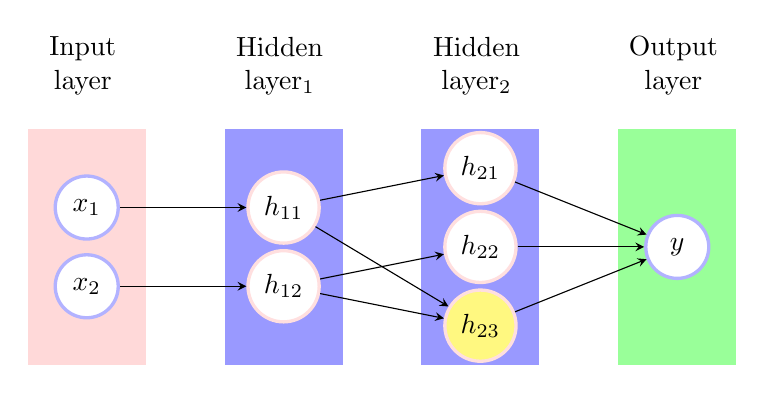
\begin{tikzpicture}
    % 结点样式名称/.style={形状,draw=颜色!色度,fill=填充色!色度,清晰度,minimum size=结点大小}
    [L1Node/.style={circle,draw=blue!30, fill=white!10, very thick, minimum size=8mm},
    L2Node/.style={circle,draw=pink!50, fill=white!10, very thick, minimum size=8mm},
    L3Node/.style={circle,draw=pink!50, fill=yellow!50, very thick, minimum size=8mm}]
    
    % 添加背景色,粉色、蓝色和绿色
    % \fill[颜色!透明度]坐标从(0,0)到(15mm,40mm)的矩形node(编号){}
    \fill[pink!60](0,0)rectangle(15mm,30mm)node(b1){};
    % \fill[颜色!透明度]坐标从(30mm,0)到(45mm,40mm)的矩形
    \fill[blue!40](25mm,0)rectangle(40mm,30mm)node(b1){};
    \fill[blue!40](50mm,0)rectangle(65mm,30mm)node(b1){};
    % \fill[颜色!透明度]坐标从(60mm,0)到(75mm,40mm)的矩形
    \fill[green!40](75mm,0)rectangle(90mm,30mm)node(b1){};
    
    % 添加输入层结点
    % \foreach循环\x依次等于1,2,3
    % \node[结点样式] (结点名称) at (结点坐标) {节点内容}
    \foreach \x in {1,...,2}
    \node[L1Node] (a_\x) at (0.75, 3-\x){$x_\x$};		
    
    % 添加隐藏层结点
    \foreach \x in {1,...,2}
    \node[L2Node] (b_\x) at (3.25, 3- \x){$h_{1\x}$};

    % 添加隐藏层结点
    \foreach \x in {1,...,2}
    \node[L2Node] (c_\x) at (5.75, 3-\x+0.5){$h_{2\x}$};

    \node[L3Node] (c_3) at (5.75, 0.5){$h_{23}$};
    % 添加输出结点
    \foreach \x in {1}
    \node[L1Node] (d_\x) at (8.25, 1.5){$y$};
    
    % 输入层到隐藏层之间的连线
    \foreach \x in {1,2}   
        % \draw[线的样式:-{stealth[sep=1pt]}为带箭头的线,[sep箭头距离]
        \draw[-stealth](a_\x)--(b_\x);
    
    \foreach \x in {1,...,2}{
    % \draw[线的样式:-{stealth[sep=1pt]}为带箭头的线,[sep箭头距离]
        \draw[-stealth](b_\x)--(c_\x);
        \draw[-stealth](b_\x)--(c_3);
    }
    \foreach \x in {1,...,3}{
    % \draw[线的样式:-{stealth[sep=1pt]}为带箭头的线,[sep箭头距离]
        \draw[-stealth](c_\x)--(d_1);
    }
    % % 隐藏层到输出层之间的连线
    % \foreach \z in{5,6,7}
    % {\foreach \y in{8}
    %     \draw[-stealth](c_\z)--(d_\y);
    % }

    % 添加说明文字
    % 名称node[居中] at (坐标) {结点内容}
    \node[align=center] at (0.7,3.8) {Input\\layer};
    \node[align=center] at (3.2,3.8) {Hidden\\layer$_1$};
    \node[align=center] at (5.7,3.8) {Hidden\\layer$_2$};
    \node[align=center] at (8.2,3.8) {Output\\layer};
\end{tikzpicture}
\vspace{5pt}
\caption{The new network structure}
\label{network1}
\end{figure}
Besides, the relationships between units in different layers are decided as follows. The yellow unit is used to transmit symbols ($+,-$).
\begin{equation}
    \begin{split}
        &h_{11} = x_1 - 1 \quad \Longrightarrow h_{11}\in\left[-1,1\right]\\
        &h_{12} = x_2 - 1 \quad \Longrightarrow h_{12}\in\left[-1,1\right]\\
        &h_{21} = h_{11} - \operatorname{sgn}\left(h_{11}\right)\cdot\frac{1}{2}\quad \Longrightarrow h_{21}\in\left[-\frac{1}{2},\frac{1}{2}\right]\\
        &h_{22} = h_{12} - \operatorname{sgn}\left(h_{12}\right)\cdot\frac{1}{2}\quad \Longrightarrow h_{22}\in\left[-\frac{1}{2},\frac{1}{2}\right]\\
        &h_{23} = h_{11}\cdot h_{12}\\
        &y = h_{21}\cdot h_{22} \cdot h_{23}
    \end{split}
\end{equation}
Thus, when $y>0$, we classify the point to positive class, and when $y<0$, we classify the point to negative class.

\vspace{4pt}
\textbf{Subproblem (3)}

As we can see, there is a recurrence process in this problem and we can get the recurrence formula 
bwtween two states as follow. We define the decision boundaries when $n=i$ as Figure \ref{rec1}, 
and then we can get decision boundaries when $n=i+1$ as Figure \ref{rec2}. Thus, we get the recurrence formula of 
the decision boundaries between state $n=i$ and state $n=i+1$ as Figure \ref{rec}, which is the regularity and global structure. Then 
we can draw the decision boundaries when the range of $x_{1}$ and $x_{2}$ to $[0,4]$ as Figure \ref{ne4}, and we can see in this situation, $n=2$.
\begin{figure}[H]
    \centering
    \subfigure[The state $n=i$]{\label{rec1}\includegraphics[width=0.25\linewidth]{images/rec1}}
    \qquad
    \subfigure[The state $n=i+1$]{\label{rec2}\includegraphics[width=0.25\linewidth]{images/rec2}}
    \caption{The recurrence formula of the decision boundaries between state $n=i$ and state $n=i+1$}
    \label{rec}
\end{figure}
\begin{figure}[H]
    \centering
    \includegraphics[width=0.5\linewidth]{images/ne4.pdf}
    \caption{The decision boundaries when the range of $x_1$ and $x_2$ to $\left[0,4\right]$}
    \label{ne4}
\end{figure}

\vspace{4pt}
\textbf{Subproblem (4)}

When the range of $x_{1}$ and $x_{2}$ is extended to $\left[0,2^{n}\right],$ the network structure is showed as Figure \ref{networkn}.

\begin{figure}[H]
    \centering
    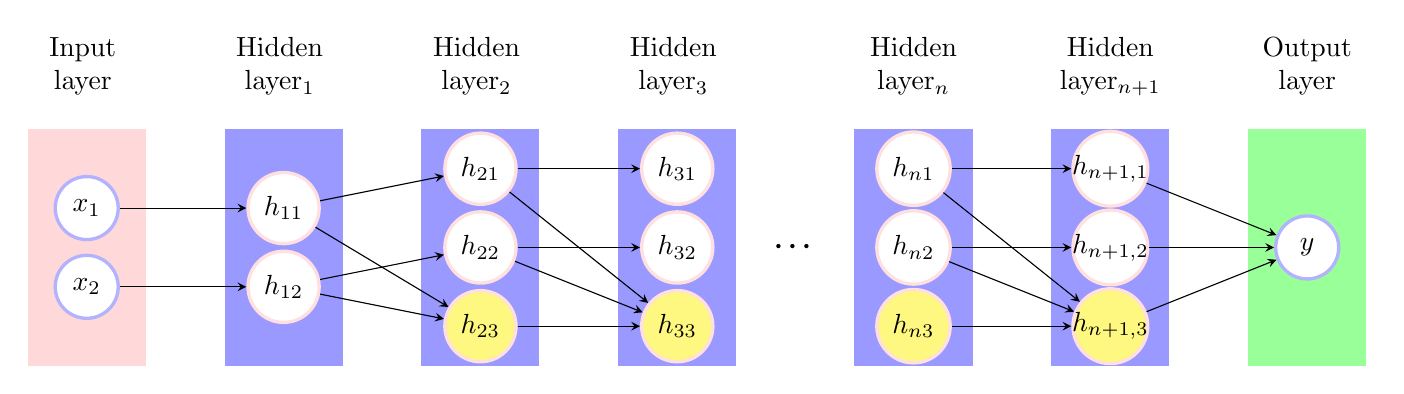
\begin{tikzpicture}
        % 结点样式名称/.style={形状,draw=颜色!色度,fill=填充色!色度,清晰度,minimum size=结点大小}
        [L1Node/.style={circle,draw=blue!30, fill=white!10, very thick, minimum size=8mm},
        L2Node/.style={circle,draw=pink!50, fill=white!10, very thick, minimum size=8mm},
        L3Node/.style={circle,draw=pink!50, fill=yellow!50, very thick, minimum size=8mm},
        L4Node/.style={circle,draw=pink!50, fill=white!10, very thick, minimum size=9.5mm},
        L5Node/.style={circle,draw=pink!50, fill=yellow!50, very thick, minimum size=9.5mm}]

        % 添加背景色,粉色、蓝色和绿色
        % \fill[颜色!透明度]坐标从(0,0)到(15mm,40mm)的矩形node(编号){}
        \fill[pink!60](0,0)rectangle(15mm,30mm)node(b1){};
        % \fill[颜色!透明度]坐标从(30mm,0)到(45mm,40mm)的矩形
        \fill[blue!40](25mm,0)rectangle(40mm,30mm)node(b1){};
        \fill[blue!40](50mm,0)rectangle(65mm,30mm)node(b1){};
        % \fill[颜色!透明度]坐标从(60mm,0)到(75mm,40mm)的矩形
        \fill[blue!40](75mm,0)rectangle(90mm,30mm)node(b1){};
        \fill[blue!40](105mm,0)rectangle(120mm,30mm)node(b1){};
        \fill[blue!40](130mm,0)rectangle(145mm,30mm)node(b1){};
        \fill[green!40](155mm,0)rectangle(170mm,30mm)node(b1){};
        % 添加输入层结点
        % \foreach循环\x依次等于1,2,3
        % \node[结点样式] (结点名称) at (结点坐标) {节点内容}
        \foreach \x in {1,...,2}
        \node[L1Node] (a_\x) at (0.75, 3-\x){$x_\x$};		
        
        % 添加隐藏层结点
        \foreach \x in {1,...,2}
        \node[L2Node] (b_\x) at (3.25, 3- \x){$h_{1\x}$};
    
        % 添加隐藏层结点
        \foreach \x in {1,...,2}
        \node[L2Node] (c_\x) at (5.75, 3-\x+0.5){$h_{2\x}$};
    
        \node[L3Node] (c_3) at (5.75, 0.5){$h_{23}$};

        % 添加隐藏层结点
        \foreach \x in {1,...,2}
        \node[L2Node] (d_\x) at (8.25, 3-\x+0.5){$h_{3\x}$};
    
        \node[L3Node] (d_3) at (8.25, 0.5){$h_{33}$};

        % 添加隐藏层结点
        \foreach \x in {1,...,2}
        \node[L2Node] (e_\x) at (11.25, 3-\x+0.5){$h_{n\x}$};
    
        \node[L3Node] (e_3) at (11.25, 0.5){$h_{n3}$};

        % 添加隐藏层结点
        \foreach \x in {1,...,2}{
        \node[L4Node] (f_\x) at (13.75, 3-\x+0.5){};
        \node[align=center] at (13.75,3-\x+0.5) {$h_{n+1,\x}$};
        }
    
        \node[L5Node] (f_3) at (13.75, 0.5){};
        \node[align=center] at (13.75,0.5) {$h_{n+1,3}$};

        % 添加输出结点
        \foreach \x in {1}
        \node[L1Node] (g_\x) at (16.25, 1.5){$y$};
        
        % 输入层到隐藏层之间的连线
        \foreach \x in {1,2}   
            % \draw[线的样式:-{stealth[sep=1pt]}为带箭头的线,[sep箭头距离]
            \draw[-stealth](a_\x)--(b_\x);
        
        \foreach \x in {1,...,2}{
        % \draw[线的样式:-{stealth[sep=1pt]}为带箭头的线,[sep箭头距离]
            \draw[-stealth](b_\x)--(c_\x);
            \draw[-stealth](b_\x)--(c_3);
        }

        \foreach \x in {1,...,2}
        % \draw[线的样式:-{stealth[sep=1pt]}为带箭头的线,[sep箭头距离]
            \draw[-stealth](c_\x)--(d_\x);
        \foreach \x in {1,...,3}
            \draw[-stealth](c_\x)--(d_3);

        \foreach \x in {1,...,2}
        % \draw[线的样式:-{stealth[sep=1pt]}为带箭头的线,[sep箭头距离]
            \draw[-stealth](e_\x)--(f_\x);
        \foreach \x in {1,...,3}
            \draw[-stealth](e_\x)--(f_3);

        \foreach \x in {1,...,3}{
        % \draw[线的样式:-{stealth[sep=1pt]}为带箭头的线,[sep箭头距离]
            \draw[-stealth](f_\x)--(g_1);
        }
        % % 隐藏层到输出层之间的连线
        % \foreach \z in{5,6,7}
        % {\foreach \y in{8}
        %     \draw[-stealth](c_\z)--(d_\y);
        % }

        %省略号
        \node[align=center] at (9.75,1.5) {$\boldsymbol{\cdots}$};
    
        % 添加说明文字
        % 名称node[居中] at (坐标) {结点内容}
        \node[align=center] at (0.7,3.8) {Input\\layer};
        \node[align=center] at (3.2,3.8) {Hidden\\layer$_1$};
        \node[align=center] at (5.7,3.8) {Hidden\\layer$_2$};
        \node[align=center] at (8.2,3.8) {Hidden\\layer$_3$};
        \node[align=center] at (11.25,3.8) {Hidden\\layer$_n$};
        \node[align=center] at (13.75,3.8) {Hidden\\layer$_{n+1}$};
        \node[align=center] at (16.25,3.8) {Output\\layer};
    \end{tikzpicture}
    \vspace{5pt}
    \caption{The network structure}
    \label{networkn}
\end{figure}
The relationships between units in different layers are decided as follows. The yellow unit is used to transmit symbols ($+,-$).

$\circ$ For input to hidden layer
\begin{equation}
    \begin{split}
        &h_{11} = x_1 - 2^{n-1} \quad \Longrightarrow h_{11}\in\left[- 2^{n-1},2^{n-1}\right]\\
        &h_{12} = x_2 - 2^{n-1} \quad \Longrightarrow h_{12}\in\left[- 2^{n-1},2^{n-1}\right]\\
    \end{split}
\end{equation}

$\circ$ For hidden layer 1 to hidden layer 2
\begin{equation}
    \begin{split}
        &h_{21} = h_{11} - \operatorname{sng}\left(h_{11}\right)\cdot 2^{n-2} \quad \Longrightarrow h_{21}\in\left[- 2^{n-2},2^{n-2}\right]\\
        &h_{22} = h_{12} - \operatorname{sng}\left(h_{12}\right)\cdot 2^{n-2} \quad \Longrightarrow h_{22}\in\left[- 2^{n-2},2^{n-2}\right]\\
        &h_{23} = h_{11}\cdot h_{12}\\
    \end{split}
\end{equation}

$\circ$ For hidden layer $i$ to hidden layer $i+1$, $i=2,3,\cdots, n$
\begin{equation}
    \begin{split}
        &h_{i+1,1} = h_{i1} - \operatorname{sng}\left(h_{i1}\right)\cdot 2^{n-i-1} \quad \Longrightarrow h_{i+1,1}\in\left[- 2^{n-i-1},2^{n-i-1}\right]\\
        &h_{i+1,2} = h_{i2} - \operatorname{sng}\left(h_{i2}\right)\cdot 2^{n-i-1} \quad \Longrightarrow h_{i+1,2}\in\left[- 2^{n-i-1},2^{n-i-1}\right]\\
        &h_{i+1,3} = h_{i1}\cdot h_{i2}\cdot h_{i3}
    \end{split}
\end{equation}

$\circ$ For the last hidden layer (hidden layer n+1) to the output layer
\begin{equation}
    \begin{split}
        &y = h_{n+1,1}\cdot h_{n+1,2} \cdot h_{n+1,3}
    \end{split}
\end{equation}
Thus, when $y>0$, we classify the point to positive class, and when $y<0$, we classify the point to negative class.

Then, we can get the complexity of computation units as follow. We define the number of units as $Q$.
\begin{equation}
    \begin{split}
        Q &= Q_{\operatorname{input}} + Q_{\operatorname{hidden}} + Q_{\operatorname{output}}\\
        &=2 + \left(n+1\right)\cdot 3 - 1 + 1\\
        &=3n+5
    \end{split}
\end{equation}
Thus, we can see the the complexity of computation units is $O\left(n\right)$.
With only one hidden layer, the network structure is specified as Figure \ref{network2}.
\begin{figure}[H]
    \centering
    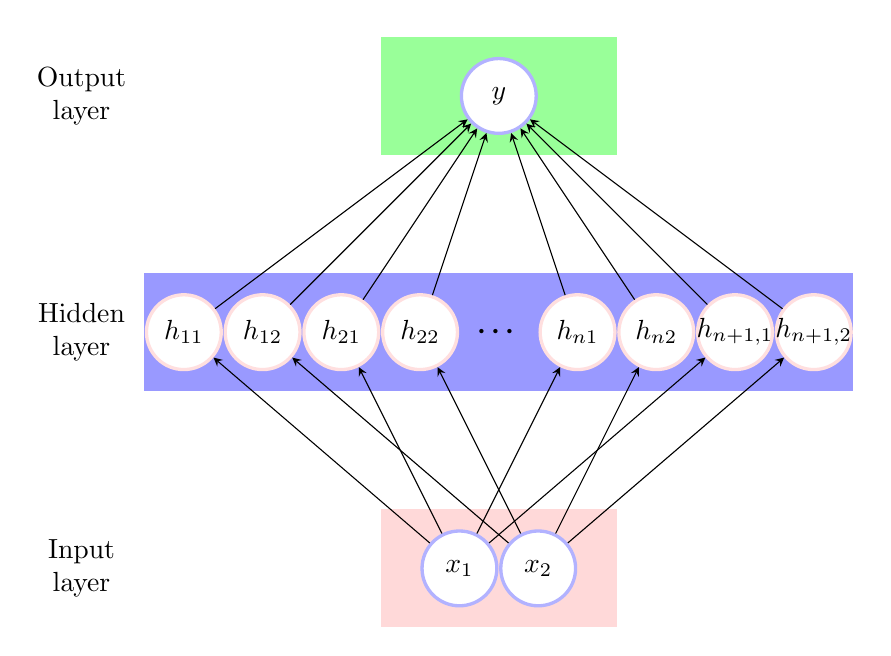
\begin{tikzpicture}
        % 结点样式名称/.style={形状,draw=颜色!色度,fill=填充色!色度,清晰度,minimum size=结点大小}
        [L1Node/.style={circle,draw=blue!30, fill=white!10, very thick, minimum size=9.5mm},
        L2Node/.style={circle,draw=pink!50, fill=white!10, very thick, minimum size=9.5mm},
        L3Node/.style={circle,draw=pink!50, fill=yellow!50, very thick, minimum size=9.5mm},
        L4Node/.style={circle,draw=pink!50, fill=white!10, very thick, minimum size=9.5mm}]
        
        % 添加背景色,粉色、蓝色和绿色
        % \fill[颜色!透明度]坐标从(0,0)到(15mm,40mm)的矩形node(编号){}
        \fill[pink!60](0,0)rectangle(30mm,15mm)node(b1){};
        % \fill[颜色!透明度]坐标从(30mm,0)到(45mm,40mm)的矩形
        \fill[blue!40](-30mm,30mm)rectangle(60mm,45mm)node(b1){};
        \fill[green!40](0,60mm)rectangle(30mm, 75mm)node(b1){};
        % \fill[颜色!透明度]坐标从(60mm,0)到(75mm,40mm)的矩形
        
        % 添加输入层结点
        % \foreach循环\x依次等于1,2,3
        % \node[结点样式] (结点名称) at (结点坐标) {节点内容}
        \foreach \x in {1,...,2}
        \node[L1Node] (a_\x) at (\x, 0.75){$x_\x$};		
        
        % 添加隐藏层结点
        \foreach \x in {1,...,2}
        \node[L2Node] (b_\x) at (-3+\x-0.5, 3.75){$h_{1\x}$};

         % 添加隐藏层结点
        \foreach \x in {1,...,2}
        \node[L2Node] (c_\x) at (-1+\x-0.5, 3.75){$h_{2\x}$};

         % 添加隐藏层结点
         \foreach \x in {1,...,2}
         \node[L2Node] (d_\x) at (2+\x-0.5, 3.75){$h_{n\x}$};

         % 添加隐藏层结点
         \foreach \x in {1,...,2}{
         \node[L4Node] (e_\x) at (4+\x-0.5, 3.75){};
         \node[align=center] at (4+\x-0.5,3.75) {$h_{n+1,\x}$};
         }
    
        % 添加输出结点
        \foreach \x in {1}
        \node[L1Node] (f_\x) at (1.5, 6.75){$y$};
        
        % 输入层到隐藏层之间的连线
        \foreach \x in {1,2}{   
            % \draw[线的样式:-{stealth[sep=1pt]}为带箭头的线,[sep箭头距离]
            \draw[-stealth](a_\x)--(b_\x);
            \draw[-stealth](a_\x)--(c_\x);
            \draw[-stealth](a_\x)--(d_\x);
            \draw[-stealth](a_\x)--(e_\x);
        }
        %省略号
        \node[align=center] at (1.5,3.75) {$\boldsymbol{\cdots}$};

        %隐藏层到输出层
        \foreach \x in {1,2}{
            \draw[-stealth](b_\x)--(f_1);
            \draw[-stealth](c_\x)--(f_1);
            \draw[-stealth](d_\x)--(f_1);
            \draw[-stealth](e_\x)--(f_1);
        }

        \node[align=center] at (-3.8,0.75) {Input\\layer};
        \node[align=center] at (-3.8,3.75) {Hidden\\layer};
        \node[align=center] at (-3.8,6.75) {Output\\layer};
    \end{tikzpicture}
    \vspace{5pt}
    \caption{The network structure with only one hidden layer}
    \label{network2}
\end{figure}

The relationships between units in different layers are decided as follows.

$\circ$ For input layer to $h_{11}, h_{12}$
\begin{equation}
    \begin{split}
        &h_{11} = x_1 - 2^{n-1} \quad \Longrightarrow h_{11}\in\left[- 2^{n-1},2^{n-1}\right]\\
        &h_{12} = x_2 - 2^{n-1} \quad \Longrightarrow h_{12}\in\left[- 2^{n-1},2^{n-1}\right]\\
    \end{split}
\end{equation}
$\circ$ For input layer to $h_{i+1,1}, h_{i+1, 2}$, $i=1, 3, \cdots, n$.
\begin{equation}
    \begin{split}
        h_{i+1,1} &= h_{i1} - \operatorname{sng}\left(h_{i1}\right)\cdot 2^{n-i-1} \,\Longrightarrow \text{we can compute it iteratively and }h_{i+1,1}\in\left[- 2^{n-i-1},2^{n-i-1}\right]\\
        h_{i+1,2} &= h_{i2} - \operatorname{sng}\left(h_{i2}\right)\cdot 2^{n-i-1} \, \Longrightarrow \text{we can compute it iteratively and }h_{i+1,2}\in\left[- 2^{n-i-1},2^{n-i-1}\right]\\
    \end{split}
\end{equation}
$\circ$ For the hidden layer to the output layer
\begin{equation}
    \begin{split}
        &y = \prod_{i=1}^{n+1} h_{i1}\cdot h_{i2}
    \end{split}
\end{equation}
Thus, when $y>0$, we classify the point to positive class, and when $y<0$, we classify the point to negative class.
\end{homeworkProblem}

\begin{homeworkProblem}
Siamese neural nets have an interesting architecture – the same parameters and functions are used to evaluate 2 inputs. As one might expect, Siamese nets are useful to train similarity metrics, evaluations of how “close” inputs are. These nets have been applied to facial recognition tasks with a good deal of success, but in this example, we’ll see how to train Siamese nets to learn a distance metric for two inputs, e.g., word vectors. One might imagine training a net to map word vectors across languages, discover synonyms or antonyms, etc.
\begin{figure}[H]
    \centering
    \includegraphics[width=0.4\linewidth]{images/snn1.png}
    \caption{The Siamese neural nets}
    \label{snn1}
\end{figure}
Here is one such model to evaluate how similar two inputs are using Euclidean distance. There are two inputs $\boldsymbol{x}_{1}, \boldsymbol{x}_{2} \in R^{n},$ shared parameters $\boldsymbol{W} \in R^{m \times n}$ and $\boldsymbol{b} \in R^{m}$, and a single hidden layer associated with each input:
$$
\begin{array}{l}
    \boldsymbol{h}_{1}=\sigma\left(\boldsymbol{W} \boldsymbol{x}_{1}+\boldsymbol{b}\right) \\
    \boldsymbol{h}_{2}=\sigma\left(\boldsymbol{W} \boldsymbol{x}_{2}+\boldsymbol{b}\right)
\end{array}
$$
We evaluate the distance between the two activations $h_{1}, h_{2}$ using Euclidean distance as our similarity metric. The model objective $\mathrm{J}$ is
$$
J=\frac{1}{2}\left\|h_{1}-h_{2}\right\|_{F}^{2}+\frac{\lambda}{2}\|W\|_{F}^{2}
$$
where $\lambda$ is a given regularization parameter. (The Frobenius norm $\|\cdot\|_{F}$ is a matrix norm defined by $\|\boldsymbol{A}\|_{F}=\sqrt{\sum_{i, j}\left|\boldsymbol{A}_{i j}\right|^{2}}$ ). The questions are as follows.
\begin{enumerate}[\quad(1)]
    \item Calculate the gradient $\nabla_{W} J$ and $\nabla_{b} J$.
    \item Write out the (vanilla) gradient descent update rules for the model parameters for a single training example (with arbitrary step size $\alpha$ ).
    \item If $\boldsymbol{W} \in R^{10 \times 5}$ and $\boldsymbol{b} \in R^{10 \times 1}$, how many parameters does the model have?
\end{enumerate}
Now imagine you wanted to see how ReLU/sigmoid nonlinearities might affect training on single input. But instead of training two separate nets, you want to train a psuedo-Siamese net like Figure \ref{snn2}.
\begin{figure}[H]
    \centering
    \includegraphics[width=0.4\linewidth]{images/snn2.png}
    \caption{The pseudo-Siamese neural nets}
    \label{snn2}
\end{figure}
The whole model would be changed to
\begin{equation}\nonumber
    \begin{split}
        &\boldsymbol{h}_{1}=\sigma\left(\boldsymbol{W}_1\boldsymbol{x}+\boldsymbol{b}_{1}\right) \\
        &\boldsymbol{h}_{2}=\operatorname{Relu}\left(\boldsymbol{W}_2\boldsymbol{x}+\boldsymbol{b}_{2}\right) \\
        &\hat{\boldsymbol{y}}=\operatorname{softmax}\left(\boldsymbol{W}_{3}\left(\boldsymbol{h}_{1}+\boldsymbol{h}_{2}\right)+\boldsymbol{b}_{3}\right)
    \end{split}
\end{equation}
where $\boldsymbol{x} \in R^{n}, \boldsymbol{W}_{1}, \boldsymbol{W}_{2} \in R^{m \times n}, \boldsymbol{W}_{3} \in R^{k \times m}, \boldsymbol{b}_{1}, \boldsymbol{b}_{2} \in R^{m}$ and $\boldsymbol{b}_{3} \in R^{k} .$ We
calculate this model for $N$ examples and $k$ classes with cross-entropy loss
$$
J=-\frac{1}{N} \sum_{j=1}^{N} \sum_{i=1}^{k} y_{j}^{i} \log \left(\hat{y}_{j}^{i}\right)
$$
where $\boldsymbol{y}_{j}$ is the one-hot vector for example $j$ with all probability mass on
the correct class and $\hat{y}_{j}$ are the softmax scores for example $j$.
\begin{enumerate}[\quad]
    \item (4) Calculate $\nabla_{\boldsymbol{h}_1} J, \nabla_{\boldsymbol{h}_2} J,$ and $\nabla_{\boldsymbol{x}} J$.
    \item (5) For $\boldsymbol{W}_{1}, \boldsymbol{W}_{2},$ which one is likely to train faster, please explain it.
\end{enumerate}

\vspace{4pt}
\textbf{\large{Solution}}

\vspace{4pt}
\textbf{Subproblem (1)}

$\circ$ For $\nabla_{\boldsymbol{W}} J$ 
\begingroup
\renewcommand*{\arraystretch}{1.5} 
\begin{equation}
    \begin{split}
        \frac{\partial J}{\partial w_{ji}}&=\frac{\partial \frac{1}{2}\left\|\boldsymbol{h}_{1}-\boldsymbol{h}_{2}\right\|_{F}^{2}}{\boldsymbol{h}_1-\boldsymbol{h}_2}\cdot\frac{\partial \left(\boldsymbol{h}_1-\boldsymbol{h}_2\right)}{\partial w_{ji}}+\frac{\partial \frac{\lambda}{2}\|\boldsymbol{W}\|_{F}^{2}}{\partial w_{ji}}\\
        &=\left(\boldsymbol{h}_1-\boldsymbol{h}_2\right)^{\top}\left(\frac{\partial \boldsymbol{h}_1}{\partial w_{ji}}-\frac{\partial \boldsymbol{h}_2}{\partial w_{ji}}\right)+\lambda w_{ji}\\
        &=\left(\boldsymbol{h}_1-\boldsymbol{h}_2\right)^{\top}
        \begin{pmatrix}
            \frac{\partial h_{11}}{\partial w_{ji}}-\frac{\partial h_{21}}{\partial w_{ji}}\\
            \frac{\partial h_{12}}{\partial w_{ji}}-\frac{\partial h_{22}}{\partial w_{ji}}\\
            \vdots\\
            \frac{\partial h_{1m}}{\partial w_{ji}}-\frac{\partial h_{2m}}{\partial w_{ji}}
        \end{pmatrix}+\lambda w_{ji}=\left(\boldsymbol{h}_1-\boldsymbol{h}_2\right)^{\top}
        \begin{pmatrix}
            0\\
            0\\
            \vdots\\
            \sigma^{'}\left(\boldsymbol{w}_j\boldsymbol{x}_1+b_j\right)\cdot x_{1i}-\sigma^{'}\left(\boldsymbol{w}_j\boldsymbol{x}_2+b_j\right)\cdot x_{2i}\\
            \vdots\\
            0
        \end{pmatrix}+\lambda w_{ji}\\
        &=\left(h_{1j}-h_{2j}\right)\cdot\left(\sigma^{'}\left(\boldsymbol{w}_j\boldsymbol{x}_1+b_j\right)\cdot x_{1i}-\sigma^{'}\left(\boldsymbol{w}_j\boldsymbol{x}_2+b_j\right)\cdot x_{2i}\right)+\lambda w_{ji}\\
    \end{split}
\end{equation}
Thus, we can get the gradient $\nabla_{\boldsymbol{W}} J$ as follow
\begin{equation}
    \begin{split}
        \nabla_{\boldsymbol{W}} J &= \left[\left(\boldsymbol{h}_1-\boldsymbol{h}_2\right)\circ \sigma^{'}\left(\boldsymbol{W}\boldsymbol{x}_1+\boldsymbol{b}\right)\right]\cdot\boldsymbol{x}_1^{\top}-
        \left[\left(\boldsymbol{h}_1-\boldsymbol{h}_2\right)\circ \sigma^{'}\left(\boldsymbol{W}\boldsymbol{x}_2+\boldsymbol{b}\right)\right]\cdot\boldsymbol{x}_2^{\top}+\lambda \boldsymbol{W}\\
    \end{split}
\end{equation}
Where $\boldsymbol{h}_1$, $\boldsymbol{h}_2$, and $\boldsymbol{b}$ are $m\times 1$ column vectors, and $\boldsymbol{x}_1$, $\boldsymbol{x}_2$ are $n\times 1$ column vectors.
\endgroup

$\circ$ For $\nabla_{\boldsymbol{b}} J$ 
\begin{equation}\nonumber
    \begin{split}
        \frac{\partial J}{\partial \boldsymbol{b}} =& \frac{\partial \frac{1}{2}\left\|\boldsymbol{h}_{1}-\boldsymbol{h}_{2}\right\|_{F}^{2}}{\boldsymbol{h}_1-\boldsymbol{h}_2}\cdot\frac{\partial \left(\boldsymbol{h}_1-\boldsymbol{h}_2\right)}{\partial \boldsymbol{b}}\\
        =&\left(\boldsymbol{h}_1-\boldsymbol{h}_2\right)^{\top}\cdot\left(\frac{\partial \boldsymbol{h}_1}{\partial \boldsymbol{b}}-\frac{\partial \boldsymbol{h}_2}{\partial \boldsymbol{b}}\right)\\
        =&\left(\boldsymbol{h}_1-\boldsymbol{h}_2\right)^{\top}\cdot\\
        &
        \begin{pmatrix}
            \sigma^{'}\left(\boldsymbol{w}_1\boldsymbol{x}_1+b_1\right)-\sigma^{'}\left(\boldsymbol{w}_1\boldsymbol{x}_2+b_1\right)&0&\cdots&0\\
            0&\sigma^{'}\left(\boldsymbol{w}_2\boldsymbol{x}_1+b_2\right)-\sigma^{'}\left(\boldsymbol{w}_1\boldsymbol{x}_2+b_1\right)&\cdots&0\\
            \vdots&\vdots&\ddots&\vdots\\
            0&0&\cdots&\sigma^{'}\left(\boldsymbol{w}_m\boldsymbol{x}_1+b_m\right)-\sigma^{'}\left(\boldsymbol{w}_1\boldsymbol{x}_2+b_1\right)
        \end{pmatrix}\\
        &=\left(\boldsymbol{h}_1-\boldsymbol{h}_2\right)^{\top}\cdot\left[\operatorname{diag}\left(\sigma^{'}\left(\boldsymbol{W}\boldsymbol{x}_1+\boldsymbol{b}\right)\right)-\operatorname{diag}\left(\sigma^{'}\left(\boldsymbol{W}\boldsymbol{x}_2+\boldsymbol{b}\right)\right)\right]
    \end{split}
\end{equation}
Thus, we can get $\nabla_{\boldsymbol{b}} J$ as follows
\begin{equation}
    \begin{split}
        \nabla_{\boldsymbol{b}} J &= \left(\frac{\partial J}{\partial \boldsymbol{b}}\right)^{\top}\\
        &=\left[\operatorname{diag}\left(\sigma^{'}\left(\boldsymbol{W}\boldsymbol{x}_1+\boldsymbol{b}\right)\right)-\operatorname{diag}\left(\sigma^{'}\left(\boldsymbol{W}\boldsymbol{x}_2+\boldsymbol{b}\right)\right)\right]\cdot \left(\boldsymbol{h}_1-\boldsymbol{h}_2\right)
    \end{split}
\end{equation}
Where $\boldsymbol{h}_1$, $\boldsymbol{h}_2$, and $\boldsymbol{b}$ are $m\times 1$ column vectors, and $\boldsymbol{x}_1$, $\boldsymbol{x}_2$ are $n\times 1$ column vectors.

\vspace{4pt}
\textbf{Subproblem (2)}

We can write out the gradient descent update rules for the model parameters for a single training example ($x_1 \text{and} x_2$) as follow
\begin{equation}
    \begin{split}
        \boldsymbol{W} &= \boldsymbol{W} - \alpha \nabla_{\boldsymbol{W}} J\\
        &=\boldsymbol{W} - \alpha \left(\left[\left(\boldsymbol{h}_1-\boldsymbol{h}_2\right)\circ \sigma^{'}\left(\boldsymbol{W}\boldsymbol{x}_1+\boldsymbol{b}\right)\right]\cdot\boldsymbol{x}_1^{\top}-
        \left[\left(\boldsymbol{h}_1-\boldsymbol{h}_2\right)\circ \sigma^{'}\left(\boldsymbol{W}\boldsymbol{x}_2+\boldsymbol{b}\right)\right]\cdot\boldsymbol{x}_2^{\top}+\lambda \boldsymbol{W}\right)\\
        \boldsymbol{b}&=\boldsymbol{b}-\alpha\nabla_{\boldsymbol{b}} J\\
        &=\boldsymbol{b} - \alpha \left(\left[\operatorname{diag}\left(\sigma^{'}\left(\boldsymbol{W}\boldsymbol{x}_1+\boldsymbol{b}\right)\right)-\operatorname{diag}\left(\sigma^{'}\left(\boldsymbol{W}\boldsymbol{x}_2+\boldsymbol{b}\right)\right)\right]\cdot \left(\boldsymbol{h}_1-\boldsymbol{h}_2\right)\right)
    \end{split}
\end{equation}

\vspace{4pt}
\textbf{Subproblem (3)}

Because $\boldsymbol{W} \in R^{10 \times 5}$ and $\boldsymbol{b} \in R^{10 \times 1}$, and there is a hyper-parameter $\lambda$, so the number of parameters in the model is
\begin{equation}
    10\times 5 + 10\times 1 + 1= 61
\end{equation}

\vspace{4pt}
\textbf{Subproblem (4)}

We have the loss function as follow
\begin{equation}
    \label{eq36}
    \begin{split}
        J&=-\frac{1}{N} \sum_{j=1}^{N} \sum_{i=1}^{k} y_{j}^{i} \log \left(\hat{y}_{j}^{i}\right)\\
        &=-\frac{1}{N} \sum_{j=1}^{N}J_j\\
        \Longrightarrow J_j &= \sum_{i=1}^{k} y_{j}^{i} \log \left(\hat{y}_{j}^{i}\right)
    \end{split}
\end{equation}
Which means that $J_j$ is the loss for the $j^{th}$ sample. Then we can compute the gradient for sample $j$. Besides, we define $\boldsymbol{\hat{y}}_j = \operatorname{softmax}\left(\boldsymbol{net}_j\right)$. We suppose that the $j^{th}$ sample belongs to the class $m$, which means $y_j^{m}=1$. Besides, we suppose $\boldsymbol{h}_1$, $\boldsymbol{h}_2$ is the vector generated by the $j^{th}$ sample.

\begingroup
\renewcommand*{\arraystretch}{1.5} 
$\circ$ For $\nabla_{\boldsymbol{h}_1} J$.
\begin{equation}
    \label{eq37}
    \begin{split}
        \frac{\partial J}{\partial \boldsymbol{h}_1} &=\frac{\partial \left(-\frac{1}{N} \sum_{j=1}^{N}J_j\right)}{\partial \boldsymbol{h}_1}\\
        &= -\frac{1}{N}\cdot\frac{\partial J_j}{\partial \boldsymbol{h}_1}\\
        &=-\frac{1}{N}\cdot\frac{\partial J_j}{\partial \boldsymbol{\hat{y}}_j}\cdot \frac{\partial \boldsymbol{\hat{y}}_j}{\partial \boldsymbol{net}_j} \cdot \frac{\partial \boldsymbol{net}_j}{\partial \boldsymbol{h}_1}
    \end{split}
\end{equation}
We can calculate $\frac{\partial J_j}{\partial \boldsymbol{\hat{y}}_j}$ as follow
\begin{equation}
    \label{eq38}
    \begin{split}
        \frac{\partial J_j}{\partial \boldsymbol{\hat{y}}_j} &= \frac{\partial \operatorname{log}\left(\hat{y}_j^{m}\right)}{\partial \boldsymbol{\hat{y}}_j}\\
        &=\begin{pmatrix}
            0&0&\cdots&\frac{1}{\hat{y}_j^{m}}&\cdots&0
        \end{pmatrix}
    \end{split}
\end{equation}
We can calculate $\frac{\partial \boldsymbol{\hat{y}}_j}{\partial \boldsymbol{net}_j}$ as follow
\begin{equation}
    \label{eq39}
    \begin{split}
        \frac{\partial \boldsymbol{\hat{y}}_j}{\partial \boldsymbol{net}_j} &= 
        \begin{pmatrix}
            &&\cdots&\cdots&&\\
            \frac{\partial \hat{y}_j^m}{\partial net_j^1}&\frac{\partial \hat{y}_j^m}{\partial net_j^2}&\cdots&\frac{\partial \hat{y}_j^m}{\partial net_j^m}&\cdots&\frac{\partial \hat{y}_j^m}{\partial net_j^k}\\
            &&\cdots&\cdots&&\\
        \end{pmatrix}\\
        &=
        \begin{pmatrix}
            &&\cdots&\cdots&&\\
            -\hat{y}_j^{1}\hat{y}_j^{m}&-\hat{y}_j^{2}\hat{y}_j^{m}&\cdots&\hat{y}_j^{m}-\left(\hat{y}_j^{m}\right)^2&\cdots&-\hat{y}_j^{k}\hat{y}_j^{m}\\
            &&\cdots&\cdots&&\\
        \end{pmatrix}\\
    \end{split}
\end{equation}
We can calculate $\frac{\partial \boldsymbol{net}_j}{\partial \boldsymbol{h}_1}$ as follow
\begin{equation}
    \label{eq40}
    \begin{split}
        \frac{\partial \boldsymbol{net}_j}{\partial \boldsymbol{h}_1}&=\frac{\partial \left(\boldsymbol{W}_{3}\left(\boldsymbol{h}_{1}+\boldsymbol{h}_{2}\right)+\boldsymbol{b}_{3}\right)}{\partial \boldsymbol{h}_1}\\
        &=\frac{\partial \left(\boldsymbol{W}_{3}\boldsymbol{h}_1\right)}{\partial \boldsymbol{h}_1} = \boldsymbol{W}_{3}
    \end{split}
\end{equation}
Then, by interesting equation \ref{eq38}, equation \ref{eq39},  and equation \ref{eq40} into equation \ref{eq37}, we can compute 
$\frac{\partial J_j}{\partial \boldsymbol{h}_1}$ as follow
\begin{equation}
    \label{eq41}
    \begin{split}
        \frac{\partial J}{\partial \boldsymbol{h}_1}&=-\frac{1}{N}\cdot\frac{\partial J_j}{\partial \boldsymbol{\hat{y}}_j}\cdot \frac{\partial \boldsymbol{\hat{y}}_j}{\partial \boldsymbol{net}_j} \cdot \frac{\partial \boldsymbol{net}_j}{\partial \boldsymbol{h}_1}\\
        &=-\frac{1}{N}\cdot
        \begin{pmatrix}
            0&0&\cdots&\frac{1}{\hat{y}_j^{m}}&\cdots&0
        \end{pmatrix}
        \cdot
        \begin{pmatrix}
            &&\cdots&\cdots&&\\
            -\hat{y}_j^{1}\hat{y}_j^{m}&-\hat{y}_j^{2}\hat{y}_j^{m}&\cdots&\hat{y}_j^{m}-\left(\hat{y}_j^{m}\right)^2&\cdots&-\hat{y}_j^{k}\hat{y}_j^{m}\\
            &&\cdots&\cdots&&\\
        \end{pmatrix}
        \cdot
        \boldsymbol{W}_3\\
        &=-\frac{1}{N}\cdot
        \begin{pmatrix}
            -\hat{y}_j^{1}&-\hat{y}_j^{2}&\cdots&1-\hat{y}_j^{m}&\cdots&-\hat{y}_j^{k}
        \end{pmatrix}
        \cdot \boldsymbol{W}_3\\
        &=-\frac{1}{N}\cdot\left(\boldsymbol{y}_j - \boldsymbol{\hat{y}}_j\right){\top}\cdot \boldsymbol{W}_3
    \end{split}
\end{equation}
\endgroup
Finally, we can get $\nabla_{\boldsymbol{h}_1} J$ as follow
\begin{equation}
    \begin{split}
        \nabla_{\boldsymbol{h}_1} J &= \left(\frac{\partial J}{\partial \boldsymbol{h}_1}\right)^{\top}\\
        &=-\frac{1}{N}\boldsymbol{W}_3^{\top}\left(\boldsymbol{y}_j - \boldsymbol{\hat{y}}_j\right)
    \end{split}
\end{equation}
Where $\boldsymbol{y}_j \text{ and } \boldsymbol{\hat{y}}_j$ are $k\times 1$ column vector.

$\circ$ For $\nabla_{\boldsymbol{h}_2} J$, it is similar to $\nabla_{\boldsymbol{h}_1} J$. Thus we can get it as follow
\begin{equation}
    \begin{split}
        \nabla_{\boldsymbol{h}_2} J &= \left(\frac{\partial J}{\partial \boldsymbol{h}_2}\right)^{\top}\\
        &=-\frac{1}{N}\boldsymbol{W}_3^{\top}\left(\boldsymbol{y}_j - \boldsymbol{\hat{y}}_j\right)
    \end{split}
\end{equation}
$\circ$ For $\nabla_{\boldsymbol{x}} J$, we consider $\boldsymbol{x}$ is the $j^{th}$ sample, as $\boldsymbol{x}_j$. Besides, in the follow equation, $\boldsymbol{h}_1$ and $\boldsymbol{h}_2$ are also generated by the $j^{th}$ sample.
\begin{equation}
    \label{eq44}
    \begin{split}
        \frac{\partial J}{\partial \boldsymbol{x}_j}&=\frac{\partial \left(-\frac{1}{N}\sum_{j=1}^{N}J_j\right) }{\partial \boldsymbol{x}_j}\\
        &=-\frac{1}{N}\cdot\frac{\partial J_j}{\partial \boldsymbol{x}_j}\\
        &=-\frac{1}{N}\cdot\left(\frac{\partial J_j}{\partial \boldsymbol{h}_1}\cdot\frac{\partial \boldsymbol{h}_1}{\partial \boldsymbol{x}_j}+\frac{\partial J_j}{\partial \boldsymbol{h}_2}\cdot\frac{\partial \boldsymbol{h}_2}{\partial \boldsymbol{x}_j}\right)\\
    \end{split}
\end{equation}
We can calculate $\frac{\partial \boldsymbol{h}_1}{\partial \boldsymbol{x}_j}$ as follows. We define $\boldsymbol{\hat{net}_j}=\boldsymbol{W}_1\boldsymbol{x}_j+\boldsymbol{b}_1$. 
\begingroup
\renewcommand*{\arraystretch}{1.5} 
\begin{equation}
    \begin{split}
        \frac{\partial\boldsymbol{h}_1}{\partial \boldsymbol{x}_j} &=\frac{\partial\boldsymbol{h}_1}{\partial \boldsymbol{net}_j^{'}}\cdot\frac{\partial\boldsymbol{net}_j^{'}}{\partial \boldsymbol{x}_j}\\
        &=\begin{pmatrix}
            \frac{\partial \sigma\left(\boldsymbol{\hat{net}}_{j,1}\right)}{\partial\boldsymbol{\hat{net}}_{j,1}}&0&\cdots&0\\
            0&\frac{\partial \sigma\left(\boldsymbol{\hat{net}}_{j,2}\right)}{\partial\boldsymbol{\hat{net}}_{j,2}}&\cdots&0\\
            \vdots&\vdots&\ddots&\vdots\\
            0&0&\cdots&\frac{\partial \sigma\left(\boldsymbol{\hat{net}}_{j,m}\right)}{\partial\boldsymbol{\hat{net}}_{j,m}}
        \end{pmatrix}
        \cdot\boldsymbol{W}_1\\
        &=\operatorname{diag}\left(\sigma^{'}\left(\boldsymbol{\hat{net}}_j\right)\right)\cdot \boldsymbol{W}_1\\
        &=\operatorname{diag}\left(\sigma^{'}\left(\boldsymbol{W}_1\boldsymbol{x}_j+\boldsymbol{b}_1\right)\right)\cdot \boldsymbol{W}_1\\
    \end{split}
\end{equation}
\endgroup
Similarly, we can get $\frac{\partial \boldsymbol{h}_2}{\partial \boldsymbol{x}_j}$ as follows.
\begin{equation}
    \begin{split}
        \frac{\partial \boldsymbol{h}_2}{\partial \boldsymbol{x}_j}
        &=\operatorname{diag}\left(\operatorname{ReLU}^{'}\left(\boldsymbol{W}_2\boldsymbol{x}_j+\boldsymbol{b}_1\right)\right)\cdot \boldsymbol{W}_2\\
    \end{split}
\end{equation}
Back to equation \ref{eq44}, we can calculate $\frac{\partial J}{\partial \boldsymbol{x}_j}$ as follow
\begin{equation}
    \begin{split}
        \frac{\partial J}{\partial \boldsymbol{x}_j}&=
        -\frac{1}{N}\cdot\left[\left(\boldsymbol{y}_j - \boldsymbol{\hat{y}}_j\right)^{\top}\cdot \boldsymbol{W}_3\cdot\operatorname{diag}\left(\sigma^{'}\left(\boldsymbol{W}_1\boldsymbol{x}_j+\boldsymbol{b}_1\right)\right)\cdot \boldsymbol{W}_1+\left(\boldsymbol{y}_j - \boldsymbol{\hat{y}}_j\right)^{\top}\cdot \boldsymbol{W}_3\cdot\operatorname{diag}\left(\operatorname{ReLU}^{'}\left(\boldsymbol{W}_2\boldsymbol{x}_j+\boldsymbol{b}_1\right)\right)\cdot \boldsymbol{W}_2\right]\\
        &=-\frac{1}{N}\cdot\left(\boldsymbol{y}_j - \boldsymbol{\hat{y}}_j\right)^{\top}\cdot \boldsymbol{W}_3\cdot\left[\operatorname{diag}\left(\sigma^{'}\left(\boldsymbol{W}_1\boldsymbol{x}_j+\boldsymbol{b}_1\right)\right)\cdot \boldsymbol{W}_1+\operatorname{diag}\left(\operatorname{ReLU}^{'}\left(\boldsymbol{W}_2\boldsymbol{x}_j+\boldsymbol{b}_1\right)\right)\cdot \boldsymbol{W}_2\right]
    \end{split}
\end{equation}
Thus, we can get $\nabla_{\boldsymbol{x}_j} J$ as follow
\begin{equation}
    \begin{split}
        \nabla_{\boldsymbol{x}_j} J &= \left(\frac{\partial J}{\partial \boldsymbol{x}_j}\right)^{\top}\\
        &=-\frac{1}{N}\cdot\left[\boldsymbol{W}_1^{\top}\operatorname{diag}\left(\sigma^{'}\left(\boldsymbol{W}_1\boldsymbol{x}_j+\boldsymbol{b}_1\right)\right)+\boldsymbol{W}_2^{\top}\operatorname{diag}\left(\operatorname{ReLU}^{'}\left(\boldsymbol{W}_2\boldsymbol{x}_j+\boldsymbol{b}_1\right)\right)\right]\cdot\boldsymbol{W}_3^{\top}\cdot\left(\boldsymbol{y}_j - \boldsymbol{\hat{y}}_j\right)
    \end{split}
\end{equation}
\vspace{4pt}
\textbf{Subproblem (5)}\\
$\boldsymbol{W}_2$ is likely to train faster. For the sigmod function, the gradient in the positive and negative saturation regions is close to 0, which may cause the vanishing gradient problem and then the training process would be very slow. 
On the contrary, for the ReLU function, it doesn't have a tendency to saturate, and there will be no particularly small gradients. Thus, the training process would be faster.
\end{homeworkProblem}
\end{document}

